% Generated by mgeoai paper-evaluate. Do not edit derived numbers manually.
\begin{table}[t]
\centering
\caption{Performance on the manually verified evaluation subset.}
\label{tab:gold-results}
\begin{tabular}{llrr}
\hline
Field & Metric & Score & $N$ \\
\hline
Fatalities & Exact match & 66.7\% & 6 \\
Fatalities & MAE & 1.6667 & 6 \\
Injuries & Exact match & 50.0\% & 2 \\
Location & Required-term agreement & 83.3\% & 6 \\
Matching & F1 & 93.6\% & 136 \\
Clustering & B-cubed F1 & 95.4\% & 17 \\
\hline
\end{tabular}
\end{table}

\begin{table}[t]
\centering
\caption{Multi-source fusion characteristics (descriptive, not accuracy).}
\label{tab:fusion-results}
\begin{tabular}{lr}
\hline
Characteristic & Value \\
\hline
Multi-source records & 49 \\
Best-single completeness & 38.6\% \\
Fused completeness & 39.1\% \\
Absolute completeness gain & 0.6\% \\
Conflict incident rate & 0.4\% \\
Provenance coverage & 100.0\% \\
\hline
\end{tabular}
\end{table}

\begin{table}[t]
\centering
\caption{Matching efficiency for the descriptive corpus run.}
\label{tab:matching-efficiency}
\begin{tabular}{lr}
\hline
Characteristic & Value \\
\hline
Theoretical cross-source pairs & 130304 \\
Candidate decisions & 5913 \\
Deterministic decisions & 5714 \\
Provider adjudications & 199 \\
Live LLM calls & 0 \\
Live-LLM call avoidance & 96.6\% \\
\hline
\end{tabular}
\end{table}

\begin{table}[t]
\centering
\caption{Geolocation representation. Country fallback markers are not incident locations.}
\label{tab:geolocation-results}
\begin{tabular}{lr}
\hline
Characteristic & Value \\
\hline
Source-named incident locations & 4 \\
Collection-country fallbacks & 437 \\
Map-marker coverage & 100.0\% \\
Incident-location coverage & 0.9\% \\
Median uncertainty radius (km) & 3.0000 \\
\hline
\end{tabular}
\end{table}

\begin{table}[t]
\centering
\caption{Observed discrepancies in the manually verified subset.}
\label{tab:error-analysis}
\begin{tabular}{lr}
\hline
Category & Count \\
\hline
location\_granularity\_disagreement & 4 \\
geographic\_disagreement & 1 \\
fatalities\_underestimate & 1 \\
injuries\_overestimate & 1 \\
fatalities\_overestimate & 1 \\
\hline
\end{tabular}
\end{table}

The manually verified subset contained 6 incidents. Among cases
with both a human fatality label and a numeric prediction, exact agreement was
66.7\%
($N=6$). Textual location agreement was
83.3\%
($N=6$). No coordinate error is reported because the
reference subset contains no trusted coordinates.

\begin{table}[t]
\centering
\caption{Automatically computed corpus characteristics (descriptive, not accuracy).}
\label{tab:corpus-results}
\begin{tabular}{lr}
\hline
Metric & Value \\
\hline
Sources & 510 \\
Evidence items & 2887 \\
Mentions & 511 \\
Fused records & 441 \\
Geolocation coverage & 0.9\% \\
Provenance coverage & 100.0\% \\
Conflict incident rate & 0.4\% \\
\hline
\end{tabular}
\end{table}

Across the automatically processed corpus, fused records exhibited an average absolute
field-completeness gain of
0.6\%
over the best single mention. This is a coverage result, not a correctness estimate.
Figures~\ref{fig:pipeline}--\ref{fig:errors} visualize the processing funnel,
modality contribution, spatial representation, and observed gold discrepancies.

\begin{figure}[t]
\centering
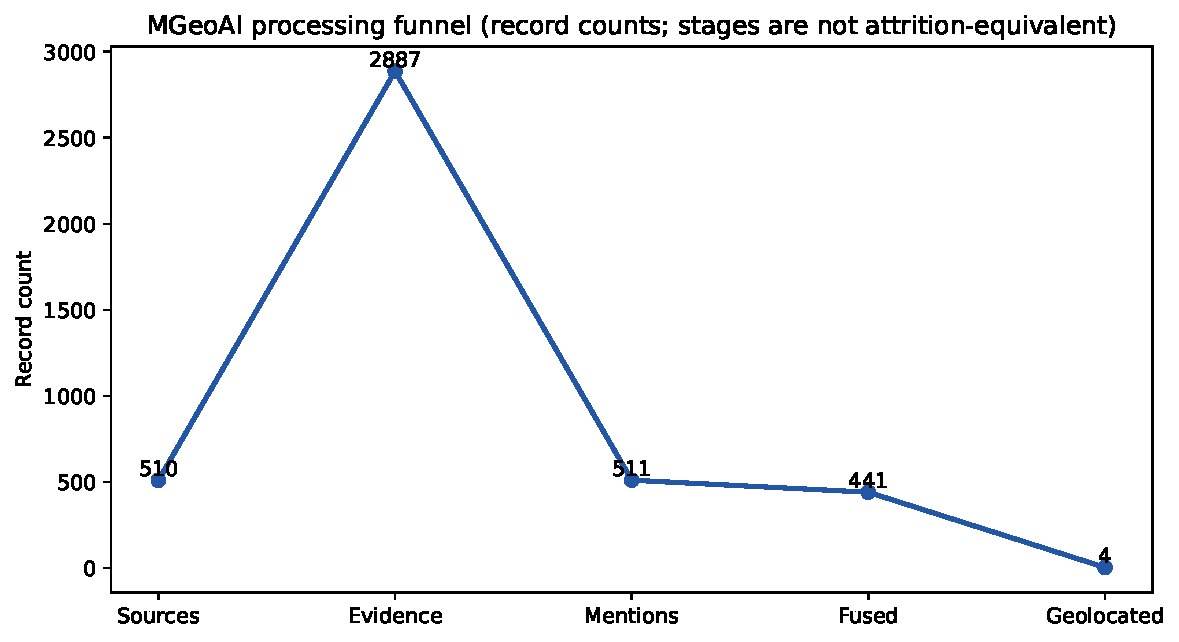
\includegraphics[width=0.95\linewidth]{evaluation/figures/figure_a_pipeline_funnel.pdf}
\caption{MGeoAI record-count processing funnel.}
\label{fig:pipeline}
\end{figure}

\begin{figure}[t]
\centering
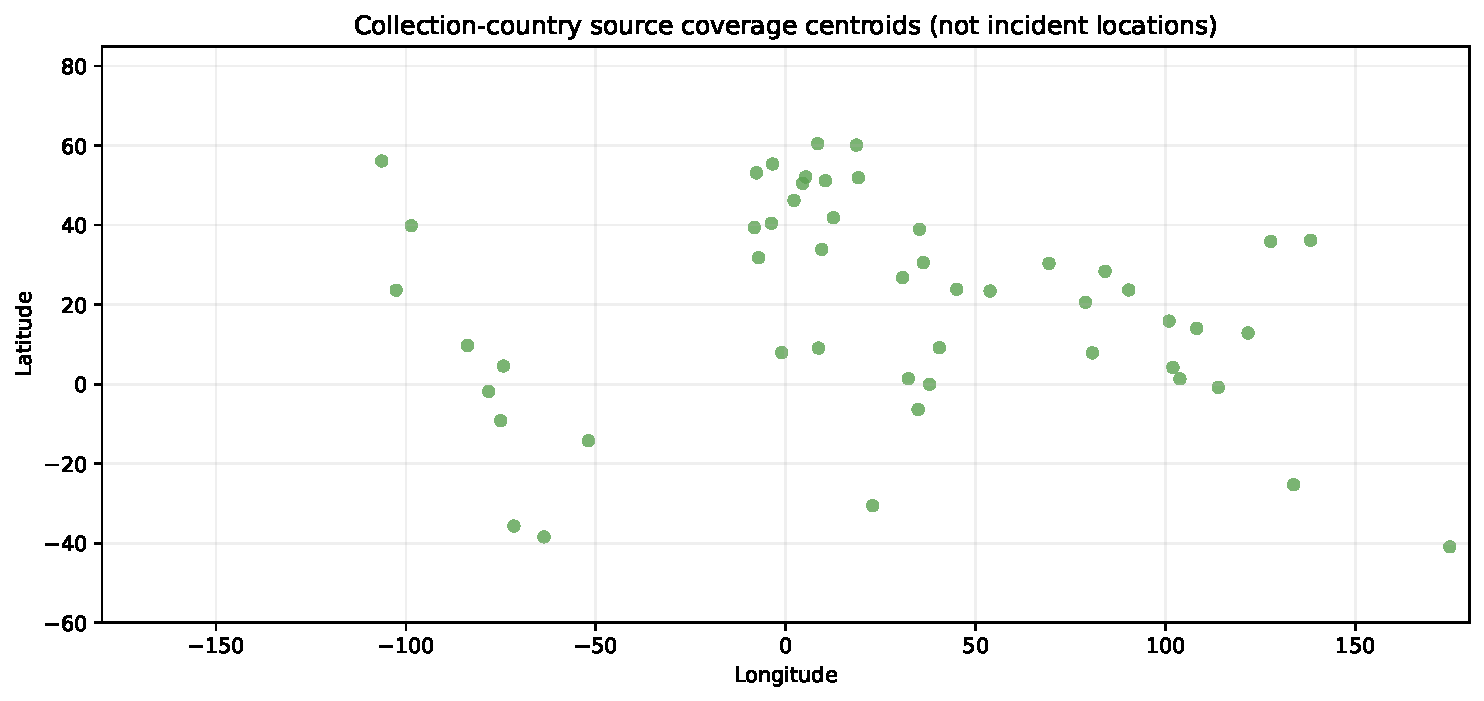
\includegraphics[width=0.95\linewidth]{evaluation/figures/figure_c_geographic_source_coverage.pdf}
\caption{Collection-country source coverage centroids; points are not incident locations.}
\label{fig:coverage}
\end{figure}

\begin{figure}[t]
\centering
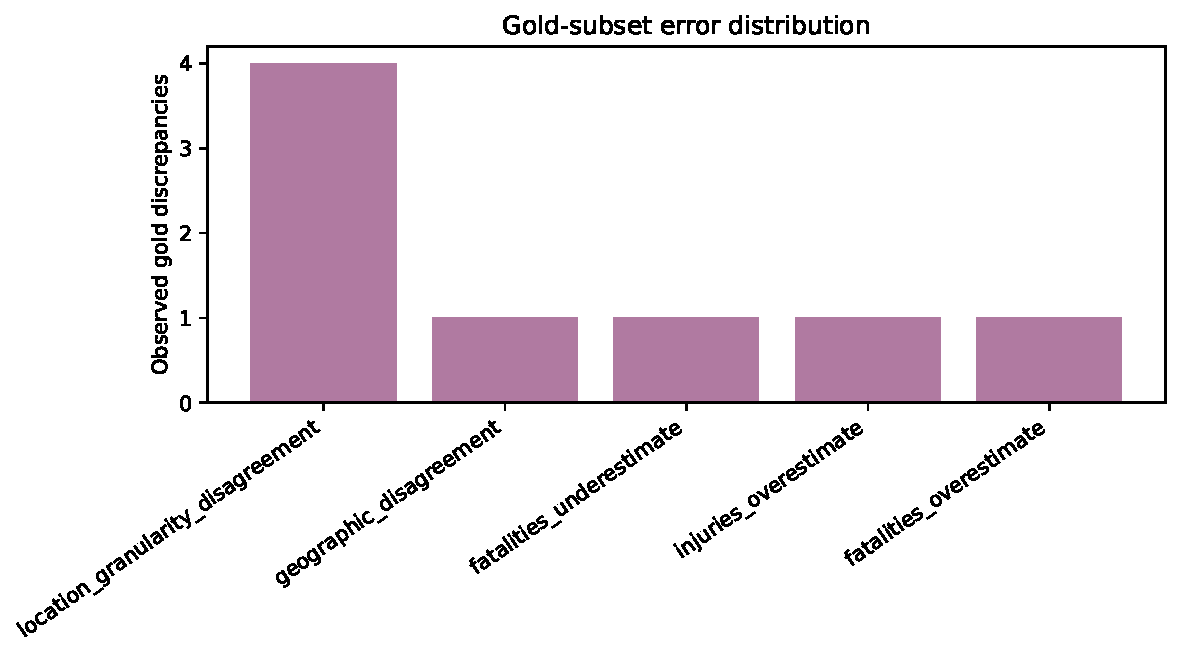
\includegraphics[width=0.95\linewidth]{evaluation/figures/figure_g_error_distribution.pdf}
\caption{Observed error categories in the manually verified subset.}
\label{fig:errors}
\end{figure}
